%%%%%%%%%%%%%%%%%%%%%%%%%%%%%%%%%%%%%%%%%
% Journal Article
% LaTeX Template
% Version 2.0 (February 7, 2023)
%
% This template originates from:
% https://www.LaTeXTemplates.com
%
% Author:
% Vel (vel@latextemplates.com)
%
% License:
% CC BY-NC-SA 4.0 (https://creativecommons.org/licenses/by-nc-sa/4.0/)
%
% NOTE: The bibliography needs to be compiled using the biber engine.
%
%%%%%%%%%%%%%%%%%%%%%%%%%%%%%%%%%%%%%%%%%

%----------------------------------------------------------------------------------------
%	PACKAGES AND OTHER DOCUMENT CONFIGURATIONS
%----------------------------------------------------------------------------------------

\documentclass[
	a4paper, % Paper size, use either a4paper or letterpaper
	10pt, % Default font size, can also use 11pt or 12pt, although this is not recommended
	unnumberedsections, % Comment to enable section numbering
	twoside, % Two side traditional mode where headers and footers change between odd and even pages, comment this option to make them fixed
]{LTJournalArticle}

\usepackage{amssymb}
\usepackage{lipsum}
\usepackage{amsthm}
\usepackage{amsfonts}
\usepackage{amsmath}
\usepackage{marvosym}
\usepackage{mathrsfs}
\usepackage{graphicx}
\usepackage{listings}
\usepackage{minted}
\usepackage{hyperref}
\graphicspath{{images/}}

\makeatletter
\renewcommand*\env@matrix[1][*\c@MaxMatrixCols c]{%
  \hskip -\arraycolsep
  \let\@ifnextchar\new@ifnextchar
  \array{#1}}
\makeatother
\newcommand*{\mbb}[1]{\mathbb{#1}}
\newcommand*{\mscr}[1]{\mathscr{#1}}
\newcommand*{\mcal}[1]{\mathcal{#1}}
\newcommand*{\R}{\mathbb{R}}
\newcommand*{\N}{\mathbb{N}}
\newcommand*{\Q}{\mathbb{Q}}
\newcommand*{\Top}{\mathcal{T}}
\newcommand*{\Rie}{\mathscr{R}}
\newcommand*{\Leb}{\mathscr{L}}
\newcommand*{\Fld}{\mathcal{F}}
\newcommand*{\der}[2]{\frac{d{#1}}{d{#2}}}
\newcommand*{\partd}[2]{\frac{\partial{#1}}{\partial{#2}}}
\newcommand*{\lto}[2]{\lim_{{#1} \to {#2}}}
\newcommand*{\dv}[1]{\,\mathrm{d}{#1}}
\newcommand*{\wbar}{\overline}
\newcommand*{\bmat}[1]{\begin{bmatrix}#1\end{bmatrix}}
\newcommand*{\angb}[1]{\langle#1\rangle}
\newcommand*{\floor}[1]{\lfloor#1\rfloor}
\newcommand*{\ceil}[1]{\lceil#1\rceil}
% upper riemann-stieltjes integral
\def\upint{\mathchoice%
    {\mkern13mu\overline{\vphantom{\intop}\mkern7mu}\mkern-20mu}%
    {\mkern7mu\overline{\vphantom{\intop}\mkern7mu}\mkern-14mu}%
    {\mkern7mu\overline{\vphantom{\intop}\mkern7mu}\mkern-14mu}%
    {\mkern7mu\overline{\vphantom{\intop}\mkern7mu}\mkern-14mu}%
  \int}
% lower riemann-stieltjes integral
\def\lowint{\mkern3mu\underline{\vphantom{\intop}\mkern7mu}\mkern-10mu\int}
\DeclareMathOperator{\Var}{Var}
\DeclareMathOperator{\sign}{sign}
\DeclareMathOperator*{\argmax}{arg\,max}
\DeclareMathOperator*{\argmin}{arg\,min}

\addbibresource{sample.bib} % BibLaTeX bibliography file

\runninghead{} % A shortened article title to appear in the running head, leave this command empty for no running head

\footertext{} % Text to appear in the footer, leave this command empty for no footer text

\setcounter{page}{1} % The page number of the first page, set this to a higher number if the article is to be part of an issue or larger work

%----------------------------------------------------------------------------------------
%	TITLE SECTION
%----------------------------------------------------------------------------------------

\title{Predicting new piano song chords using Tonnetz graphs and CNNs (ECE 227 project)} % Article title, use manual lines breaks (\\) to beautify the layout

% Authors are listed in a comma-separated list with superscript numbers indicating affiliations
% \thanks{} is used for any text that should be placed in a footnote on the first page, such as the corresponding author's email, journal acceptance dates, a copyright/license notice, keywords, etc
\author{%
	Jerry Yan\textsuperscript{1} (A15881043)
}

% Affiliations are output in the \date{} command
\date{\footnotesize\textsuperscript{\textbf{1}}Department of Electrical and Computer Engineering, University of California San Diego}

% Full-width abstract
\renewcommand{\maketitlehookd}{%
	\begin{abstract}
		\noindent In this project, we analyze the effectiveness of Tonnetz graphs as representations of piano music, and whether they can be used to predict new music. We will look at completely synthetic methods of chord production, namely using cellular automaton, as well as data driven methods using convolutional neural networks. The direct utilization of the 2D representation of music allows for the usage of many processing techniques from other fields, namely image processing. This paper will test the feasibility of such methods to predict the chords of a song and even synthesize new music past the end of a score.
	\end{abstract}
}

%----------------------------------------------------------------------------------------

\begin{document}

\maketitle % Output the title section

%----------------------------------------------------------------------------------------
%	ARTICLE CONTENTS
%----------------------------------------------------------------------------------------

% note: how to cite \textcite{job_openings_fall}
\section{Introduction}

AI generated media has recently seen numerous advancements in the fields of large language models and generative art/photos. In this paper however, we focus on the synthesis of music, which has also seen recent breakthroughs, such as the text-prompt generative model \hyperlink{https://suno.com/}{Suno AI}.

This paper does not explore the general synthesis of music, but instead focuses on piano songs, and creating new measures of tonal chords by modeling a whole songs as a series of Tonnetz graphs (\textcite{tymoczko_generalized_2012}). At the core of songs in general, they usually follow particular chord progressions that are broken up in different ways. Many melodies and basslines can simplify to chords split up and played in different orders and tempos. Of course, music in its entirety is much more complicated than that, and entire genres of music have been build around particular chord progressions and tempos (\textcite{pressing_black_2002}). Other similar studies have also tried to embed songs in the space of Tonnetz graphs to predict new song chords (\textcite{aminian_exploring_2020}), but do not use the Tonnetz graph representation directly in the model (the Tonnetz graph is used to embed chords into a new vector space), and use different kinds of models (a LSTM model in the other paper's case). Other studies have shown methods of learning chord embeddings (\textcite{madjiheurem_chord2vec_2016}) without any prior knowledge of tonal and harmonic chords, which in a vacuum would prove more effective if we didn't already have existing knowledge of tonal relationships.

In terms of using CNNs on audio data, previous work has explored the classification of audio using CNNs (\textcite{hershey_cnn_2017, palanisamy_rethinking_2020}) by using various representations of audio data. This ranges from just convolving over the original waveform audio data, or into other formats of data, such as spectrograms or chromagrams, which are 2D representations of audio, allowing a 2D convolution. However, no previous literature (I couldn't find any) attempted to process a Tonnetz graph representation of songs directly. Obviously for general audio data, these formats are more suitable, but for music and especially piano music, the fact we can work directly with individual notes means there is insight that can be learned within Tonnetz graphs.

In later sections of the paper, we will discuss music generated purely synthetically without data using cellular automaton rules. In particular Conway's Game of Life (\textcite{bays_introduction_2010}) will be used to generate piano chords. We will then analyze the effectiveness of embedding piano chords into Tonnetz graphs instead of just vectorizing the chords, and test how convolution neural networks (CNNs) perform on the task of generating new chords.

\section{Background}

\subsection{Dataset used}

We use the GiantMIDI-Piano dataset (\textcite{kong_giantmidi-piano_2022}) for training and testing our models. Since the audio data is in the MIDI file format, we can extract individual notes from every song and when they are played.

\subsection{Tonnetz graph}

The Tonnetz graph (\textcite{tymoczko_generalized_2012}) is an infinite planar lattice graph that models tonal relationships between musical notes. There are several intervallic structures that can model different tonal relations between notes, but the most commonly used is the triad 3-4-5 representation of notes. In other words, every edge represents either a major 3rd, 4th, or 5th interval. A visualization of the 3-4-5 Tonnetz graph is found in \autoref{fig:tonnetz}. Different patterns of notes can represent different types of chords, such as major, minor, augmented chords, etc. A more detailed relation between notes and their neighbors is provided in \autoref{fig:tonnetz-c4neigh}. From now onwards, since every note has exactly six neighboring notes, we will be representing the Tonnetz graph as a hexagonal grid.

Since the Tonnetz graph itself has inherent tonal relationships between notes with respect to spatial relation, it has the advantage of already modeling that information when representing the music as data, and thus relationships between each notes do not necessarily need to be learned.

The infinite nature of the Tonnetz graph is problematic when attempting to represent songs, so we have to limit representations of chords to a finite subgraph of the Tonnetz. Since we are working with piano music, we can limit the number of notes to the 88 keys on the standard piano (\autoref{fig:tonnetz-finite}). This is a $13\times9$ graph when stored in a rectangular grid.

\begin{figure}
    \centering
    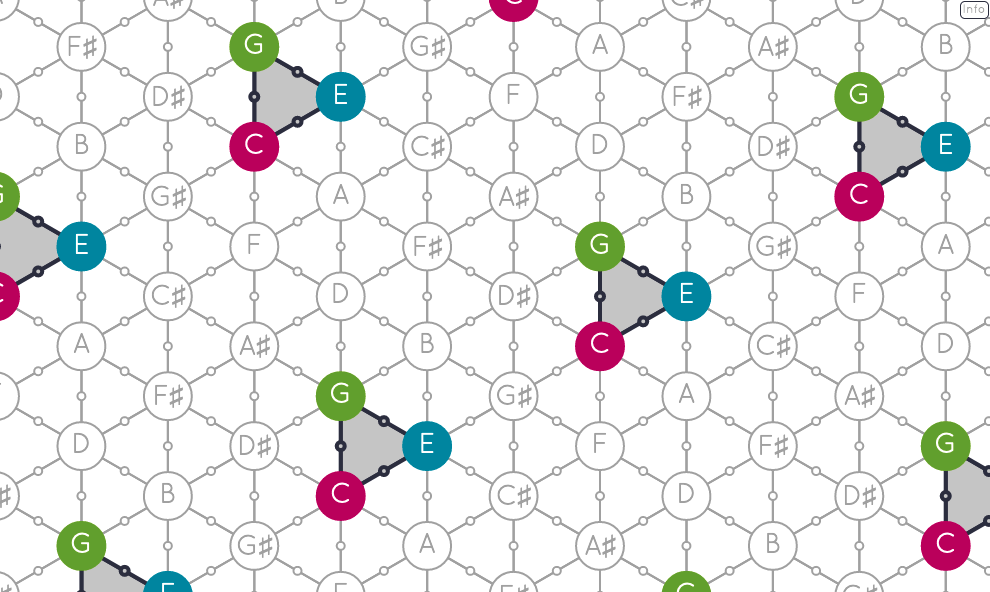
\includegraphics[width=\linewidth]{images/tonnetz-webhex.png}
    \caption{A visualization of a 3-4-5 Tonnetz graph. The highlighted notes represent a C-major chord. In fact, all major chords will take this shape. Also note that each note here takes a different octave, though it is not labeled. Figure from \href{https://guichaoua.gitlab.io/web-hexachord/}{HexaChord}.}
    \label{fig:tonnetz}
\end{figure}

\begin{figure}
    \centering
    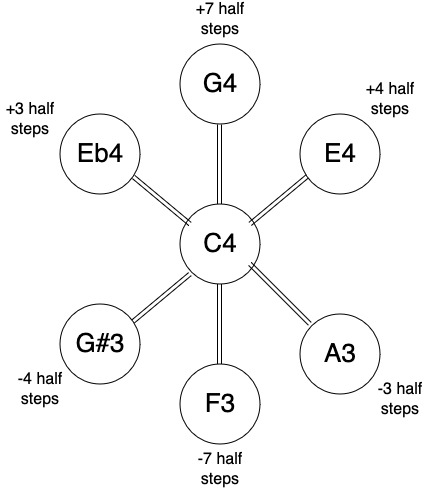
\includegraphics[width=0.8\linewidth]{images/tonnetzC4.jpg}
    \caption{A visualization of the relationship between notes in a 3-4-5 Tonnetz graph by looking at the neighbors of middle C (C4). A half step is the smallest possible interval between two notes.}
    \label{fig:tonnetz-c4neigh}
\end{figure}

\begin{figure}
    \centering
    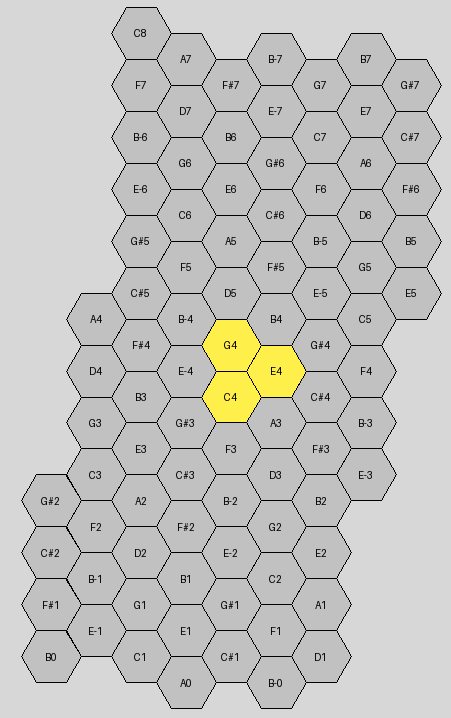
\includegraphics[width=0.8\linewidth]{images/tonnetz-finite.png}
    \caption{The finite 88-key subgraph of the Tonnetz that will be used in our models. The highlighted yellow notes are currently being played, and in this case represents a middle C-major chord.}
    \label{fig:tonnetz-finite}
\end{figure}

\subsection{Conway's Game of Life}

Conway's Game of Life (\textcite{bays_introduction_2010}) is an example of a cellular automaton, where we have a grid of cells that are either alive or dead. Then according to a set of rules, we change the state of each cell to represent the next generation of cells. Traditionally, Conway's Game of Life is played on a square grid, where each cell has 8 neighbors. A live cell will survive if it has exactly 2 or 3 live neighbors, otherwise it dies. A dead cell will give birth to a new live cell if it has exactly 3 live neighbors. These numbers are arbitrary, and different values will result in vastly different behaviors.

The game of life can be generalized to any 2D grid, and in our case, we will use a hexagonal grid, so that each cell will only have 6 neighbors. The game of life has been widely studied and example animations can be found on \href{https://en.wikipedia.org/wiki/Conway%27s_Game_of_Life}{Wikipedia}.

\subsection{Convolutional networks and segmentation}

The 2D segmentation problem is a classification problem where given a 2D grid of data, it predicts which class each grid cell belongs to. In our case, this becomes a binary segmentation problem where a note on the Tonnetz grid is either active (being played) or inactive. Convolutional neural networks are the standard models for solving this problem. The methodology section will go into further detail on how we will represent this chord prediction problem as a segmentation problem.

When processing and learning from data represented as 2D grid structures (e.g. images), 2D convolutions are used to learn 2D spatial relations between each cell in the data. Since we are dealing with a different grid type than the usual rectangular grid, we have to use special hexagonal kernels to convolve our Tonnetz graphs (\textcite{luo_hexagonal_2019}), as visualized in \autoref{fig:hex-conv}.

\subsubsection{U-Net}

One of the most widely used segmentation CNNs is U-Net (\textcite{ronneberger_u-net_2015}), whose architecture can be found in \autoref{fig:unet-arch}. As a summary of how the model works, it first encodes the image by downsampling the image using convolutional and max pooling layers, then upsampling with convolutions. At each downsampling level, a skip connection copies the result to its corresponding upsampling level in order to preserve original information about the input image.

\begin{figure}
    \centering
    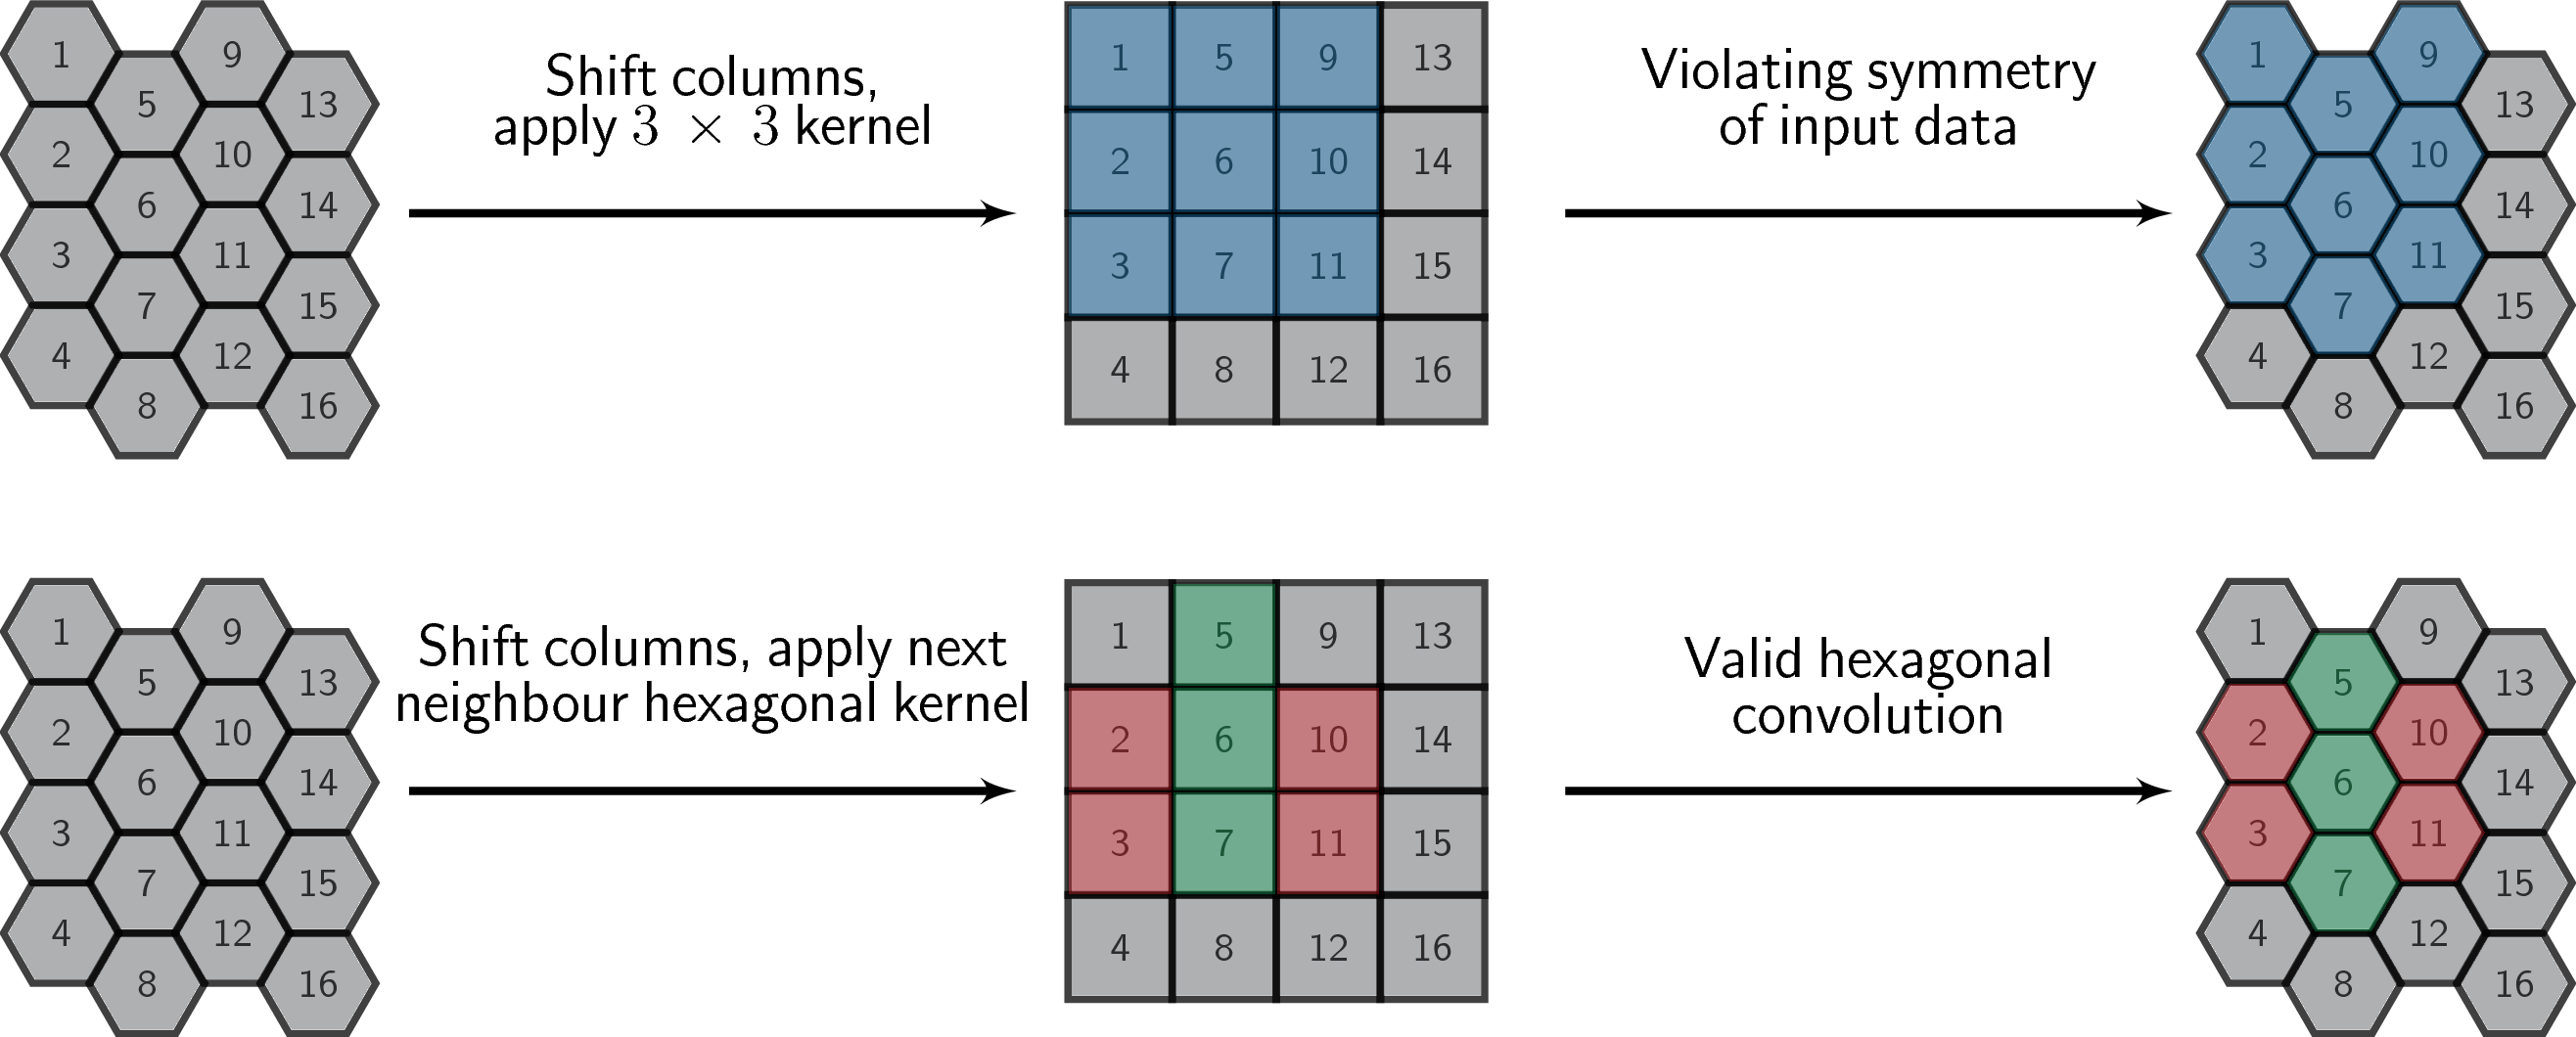
\includegraphics[width=\linewidth]{images/violating_symmetry.png}
    \caption{A comparison between usual square kernels and hexagonal kernels. A square kernel would incorrectly convolve the neighbors of a hexagonal cell, so a special kernel must be used. Figure from \textcite{luo_hexagonal_2019}.}
    \label{fig:hex-conv}
\end{figure}

\begin{figure}
    \centering
    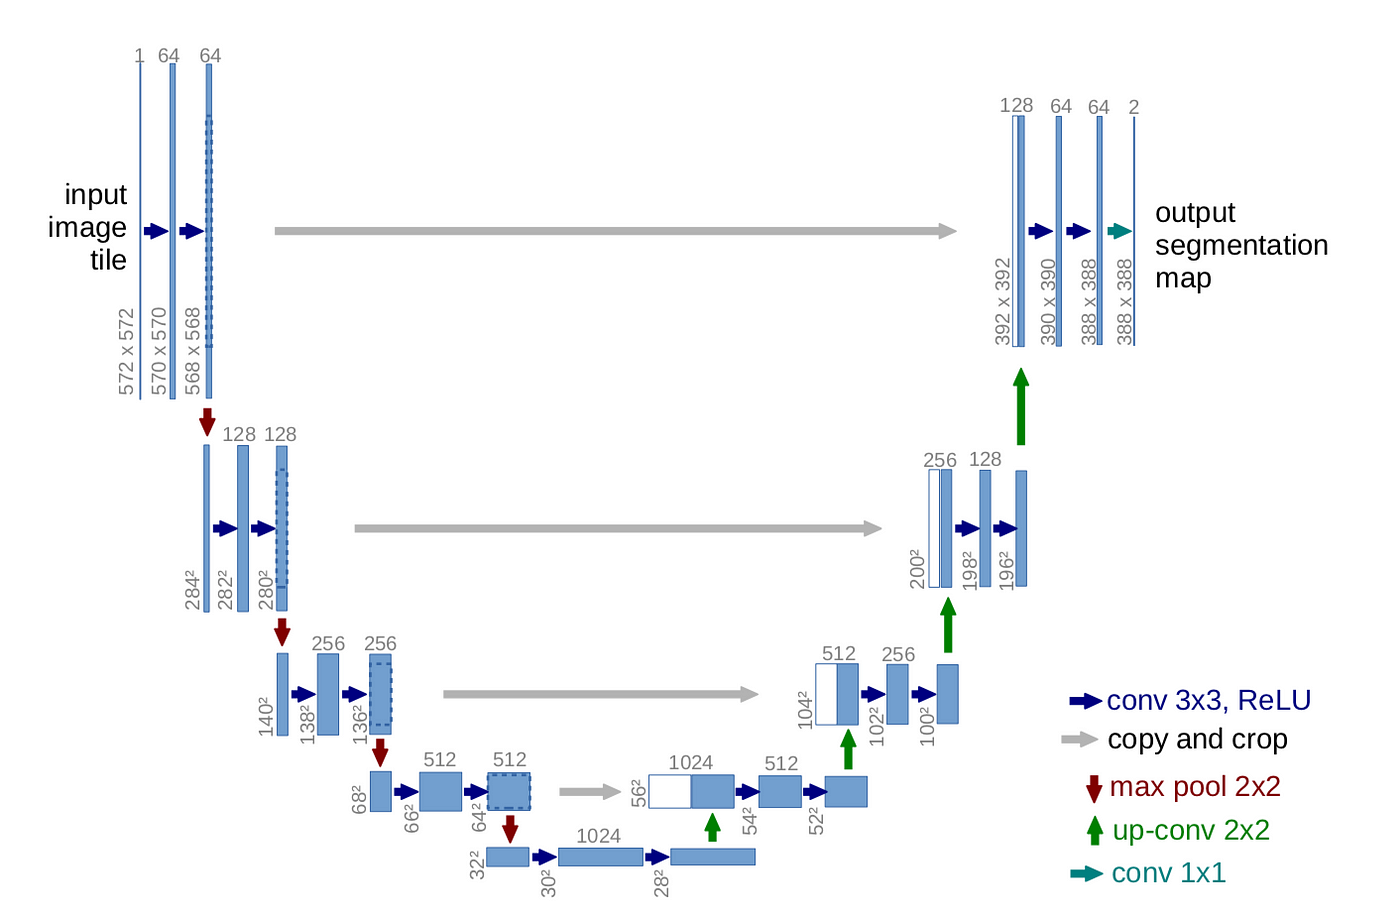
\includegraphics[width=\linewidth]{images/unet-arch.png}
    \caption{Architecture of U-Net, from \textcite{ronneberger_u-net_2015}.}
    \label{fig:unet-arch}
\end{figure}

\subsection{Other embeddings of chords}

Another known embedding of chords in a new feature space is one-hot encoding each chord as shown in \texttt{chord2vec} (\textcite{madjiheurem_chord2vec_2016}). This method functions very similarly to the \texttt{word2vec} model (\textcite{mikolov_efficient_2013}), where the model attempts to learn chord representations to predict temporally neighboring chords in a given musical score. A single chord is represented as a "many-hot" vector where each active element in the vector is the note played. Due to limited time however, I will not be testing these embeddings and their performances.

\section{Methodology}

\subsection{Songs from cellular automaton}

In our implementation of a hexagonal game of life, we will essentially treat every live cell as a played note. For the sake of simplicity and sanity of the generated notes, every generation and its live cells will represent a single chord in the song, and these chords will be played sequentially. Since the game of life is supposed to be simulated on an infinite grid, we will let the live cells expand out of our 88-key finite Tonnetz graph, as shown in a snapshot of one of the generations \autoref{fig:gameoflife-gen16}. In our particular example, we play with the rules that a dead cell is birthed if it has exactly 2 neighbors, and a live cell only survives if it has exactly 1 or 2 neighbors.

\begin{figure}
    \centering
    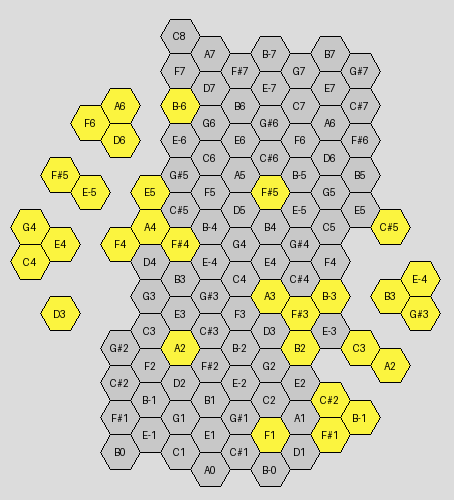
\includegraphics[width=0.9\linewidth]{images/gameoflife-gen16.png}
    \caption{A snapshot of generation 16 of game of life, where our first live cells were notes E-4 and C4. We can observe a number of major and minor chords being played simultaneously.}
    \label{fig:gameoflife-gen16}
\end{figure}

\subsection{Representing songs as a Tonnetz series}

Since most songs usually follow particular chord progressions that are broken up in different ways, we will simplify songs by consolidating notes temporally. The time interval in which we consolidate notes is arbitrary, and the best interval to use will depends on the song. We can choose eighth, quarter, half, or whole intervals to discretize the song into separate chords. For example, fast songs with rapid scales and arpeggios can retain a higher resolution of chords during synthesis by choosing a smaller scale. If there are time intervals where no notes are played, we simply ignore them and skip to the next timestep that notes are played for the sake of simplicity, so any discretized song will be shorter than the original (\autoref{fig:score-discrete}). We do not differentiate between melodic and harmonic notes since that distinction is not provided in our MIDI file data.

Then since we have grouped notes together into chords at set timestamps, we can then store each of these chords into separate Tonnetz graphs, where the notes in the chords are active in the graph, so we end up with a time series of Tonnetz graphs. Then the graphs represent the evolution of chords temporally for a specific song.

\begin{figure}
    \centering
    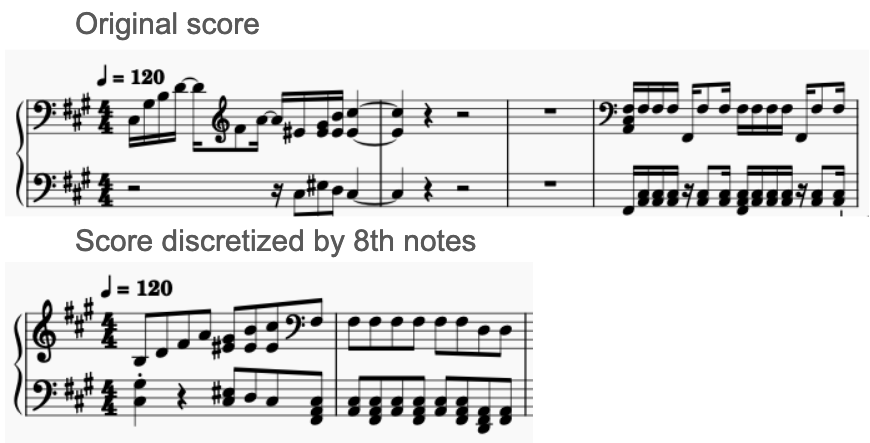
\includegraphics[width=\linewidth]{images/score-discrete-gerudo.png}
    \caption{An example of the discretization of a piano score into eighth notes. Note the rests are removed, so the song is shortened. This song is the beginning of the piano transcription of the Gerudo Valley theme, found on \href{https://www.ninsheetmusic.org/browse/series/TheLegendofZelda}{NinSheetMusic}.}
    \label{fig:score-discrete}
\end{figure}

\subsection{Chord prediction as a segmentation problem}

Performing segmentation on our Tonnetz graph series is highly unconventional compared to the tasks segmentation is usually used for. Instead of inputting a 3-channel image, we will be using an $c$-channel series of finite Tonnetz graphs, where we will be using the previous $c$ chords to predict the next single chord. As mentioned previously, our Tonnetz graph can be stored on a $13\times9$ grid, so our input data have the dimension $c\times13\times9$. Due to the sparsity of the graphs in some measures, the chosen $c$ might depend on the song and interval chosen, since if we only choose $c=1$, and the previous chord played was just a single note, there is not much we can do with a single active cell. In fact, the graph even has a chance to vanish if depending on our convolutional layer training (where no notes are played).

We also note that every Tonnetz graph will only hold one of 2 cell values: active or inactive, and we want to predict which notes would be active/inactive in the next timestep. We can continuously generate music by then feeding the output mask back into the input to predict new chords. We remove the oldest chord in the input and put the new predicted chord at the end of our input tensor as the last channel. In summary, we are using a series of binary masks and predicting a new binary mask, making this a departure from traditional segmentation problems.

This unique problem also runs into a situation where between each training pair is highly correlated with other training pairs, since for each $c\times13\times9$ input and a $1\times13\times9$ output, that output will then be included in the $c$ subsequent training pairs as input. This will limit how we can split our data for training and validation.

\subsubsection{Training and data split}

In this problem with predicting musical chords, there is no definitive way to choosing how to partition the data and which songs to train a network on, since we can use different training sets for entirely different purposes. If we want to extend a single song, or synthesize something in the style of a specific song, we are only able to use a single song as training data. This means there is not much data to work with, but any model fit to the song will very reliably produce chords sounding like the original song. Unfortunately this also means splitting a song into a training and test set is basically useless, since the split means there is barely any test data, and that all our data is already highly correlated. Every test point will bear high similarity to a training point due to the overlap of our data. If we train a network song-by-song, our only way to evaluate it would be training error.

We could also choose a single artist and all the artist's songs as training data if we want to create chords of their style. This makes the network a lot more general and much less tailored to a specific style of song. However, our experiments will focus song-by-song training since I personally find it more interesting.

In our later experiments, we explicitly work by discretizing songs into quarter intervals, and working with $c=4$.

\subsubsection{Model 1: simple convolutional neural network}

As a benchmark, we use a network that is made purely of convolution and ReLU layers, without any downsampling or skip connections, to see if convolutions by themselves can capture song behavior. This network has convolutions going from $c\to64\to128\to64\to1$ channels, with a ReLU in between each convolution layer. Note that no max pooling exists in this network.

\subsubsection{Model 2: Culled U-Net}

Due to the fact each finite Tonnetz grid is only $13\times9$, the amount of downsampling layers in the standard version of U-Net will make the image vanish. In addition, the sample space of possible Tonnetz graph configurations is magnitudes smaller than traditional image data, so it is preferable in theory to cut down on the number of layers. Instead of the 4 downsample/upsample pairs in the original architecture (\autoref{fig:unet-arch}), we cut it down to only 2 pairs (we only convolve up to 256 channels), while keeping the skip connections. In other words, we use a shallower U-Net.

\subsubsection{Evaluation of performance}

Since this is a binary segmentation problem, we use weighted binary cross entropy loss to train our networks. For a particular Tonnetz cell predicted/truth pair $(x_{i,j},y_{i,j})$, it is defined as

\begin{equation}
    l_{i,j} = -[py_{i,j}\ln\sigma(x_{i,j}) + (1-y_{i,j})\ln(1-\sigma(x_{i,j}))]
\end{equation}

where $\sigma$ is our sigmoid activation function and $p$ is a weight we give to all positive data points to increase either recall ($p>1$) or precision ($p<1$). For a whole predicted Tonnetz graph, we consolidate the loss of every cell in the graph by averaging them.

\begin{equation}
\ell_n = \frac{1}{88}\sum_{i,j}l_{i,j}
\end{equation}

Since each Tonnetz graph is very sparse (we only have 10 fingers, so there's only so many notes at one timestep), we will increase $p>1$, or else the network will tend towards predicting every note as unplayed. I arbitrarily chose $p=5$ because I couldn't be bothered to calculate a value more rigorously.

For human readable interpretation of performance, we will simply use $F_\beta$ score with $\beta=2>1$ since we value recall higher.

\begin{equation}
    F_\beta = (1+\beta^2)\frac{\text{precision}\cdot\text{recall}}{(\beta^2\cdot\text{precision})+\text{recall}}
\end{equation}

There are actually two distinct ways to evaluate the performance of our network: we can calculate metrics for each predicted chord individually by generating them from the input chords separately, or we can give the network the initial chords, and let it continuously generate chords for $T$ timesteps, and then compare it to the original training data. We will look at the performance of both of these methods.

\section{Results and discussion}

\subsection{Game of life results}

There's not much to evaluate or discuss on the results of cellular automaton simulations, since depending on the initial pattern, it either cycles, vanishes, or explodes in the number of notes being played. In \autoref{fig:gameoflife-midi}, we can see an example of the number of notes exploding to the point where it's basically incomprehensible after a few generations. Even if we split the notes up into a melody, it would still sound chaotic.

\begin{figure*}
    \centering
    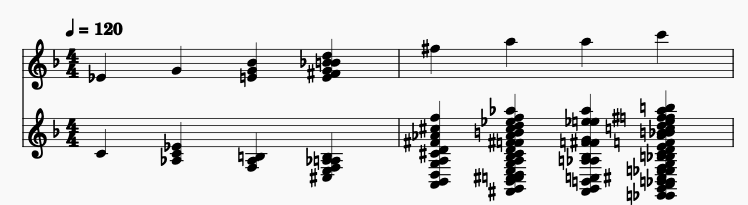
\includegraphics[width=0.7\linewidth]{images/gameoflife-midi.png}
    \caption{The first 8 generations from game of life on the Tonnetz graph, where each generation is a quarter note. We can see the first 3 chords do generate as standard tonal chords, but they quickly devolve into illegible chaos.}
    \label{fig:gameoflife-midi}
\end{figure*}

\subsection{CNN results}

We evaluate for both individually generated chord performance and continuous generation performance, as seen in \autoref{tab:cnn-metrics}. In both cases, we start off with 4 initial chords in the beginning of the song, and generate chords for 100 generations, with each new chord being fed back into the 4 input chords. We perform this test for only 100 songs for the sake of sanity.

\begin{table}
	\caption{Metrics of 100 models tested on 100 different songs with $c=4$ and quarter intervals (there were 10000 songs in the dataset, I'm not testing them all). Each metric is the average between all 100 models. The average train loss (binary cross entropy)/F2 measure how well each $c=4$ previous chords predict the next chord. The 100 chord F2 measures how well the next 100 chords are reconstructed from only $c=4$ initial chords.}
	\centering
	\begin{tabular}{|c||c|c|} 
     \hline
     Model & Simple CNN & U-Net \\
     Metrics && \\
     \hline\hline
     Avg train loss & 0.222 & 0.072 \\ 
     \hline
     Avg train F2 & 0.65 & 0.929 \\
     \hline
     Avg F2 (100 chords) & 0.31 & 0.3 \\
     \hline
    \end{tabular}
	\label{tab:cnn-metrics}
\end{table}

\begin{figure}
    \centering
    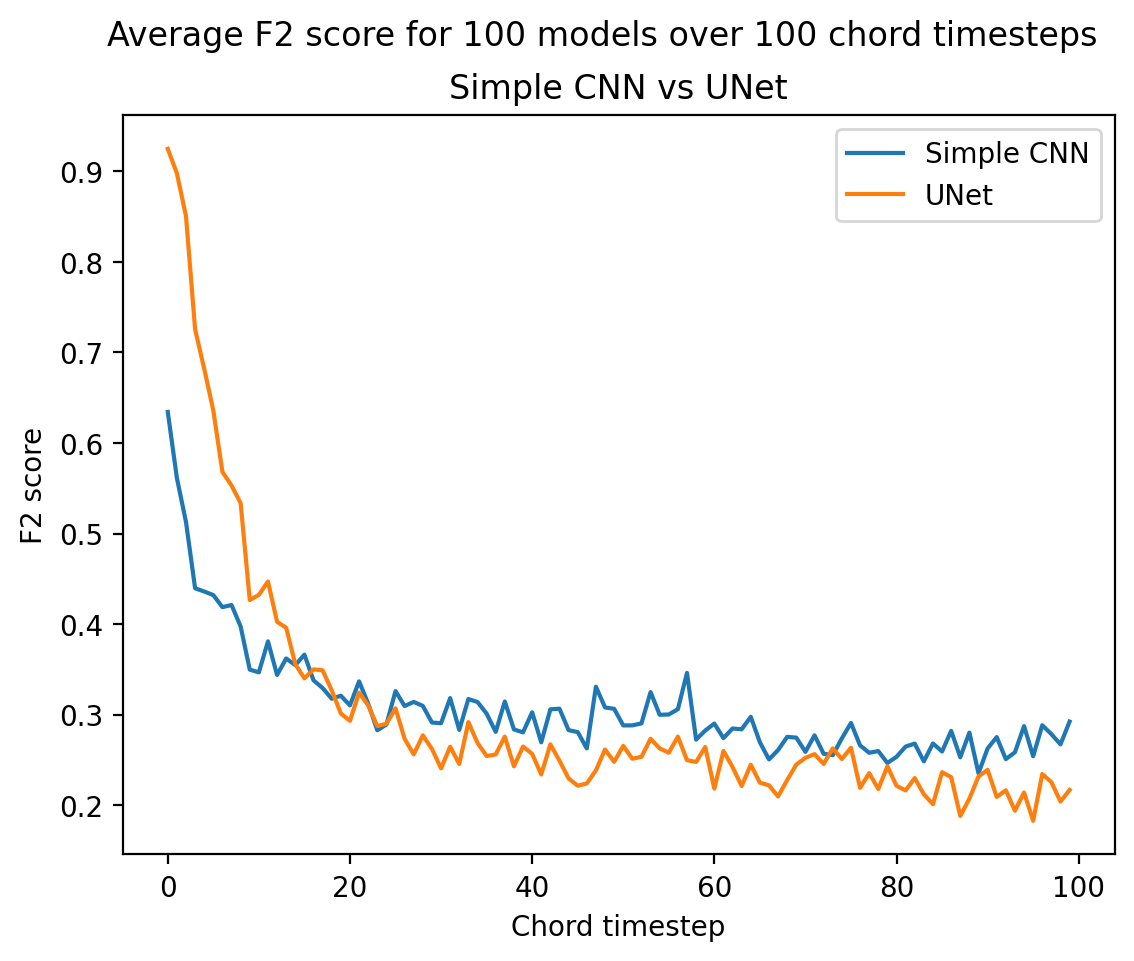
\includegraphics[width=\linewidth]{images/simplecnnvsunet.png}
    \caption{The F2 scores of the chords over time by repeatedly feeding predicted chords back into the network for 100 timesteps. As expected, the further from the initial chords we get, the accuracy of the chords rapidly decreases.}
    \label{fig:cnn-comp}
\end{figure}

\subsubsection{Simple CNN results}

In terms of pure performance, the simple CNN performs well compared to simply randomly choosing notes (trivially, the probability of choosing the correct notes for a chord randomly is vastly less than 0.1) with an F2 score of 0.65 (\autoref{tab:cnn-metrics}). When continuously generating chords, we can see its performance drop significantly, but is still better than generating randomly. In the timeseries in \autoref{fig:cnn-comp}, we can see expectedly that the F2 score between the predicted and true chords rapidly drops as we generate more notes, since predicting chords based off predicted chords will become unreliable quickly, just like most forecasts.

However, numbers do not tell the whole story of how a network performs. When the CNN operates on our Tonnetz graphs repeatedly by feeding itself its own inputs, we are essentially performing infinite convolutions on the input, while including activation functions in between.

\begin{equation}
\begin{split}
    f_T = & f * \sigma(f) \circ \sigma(f) \circ \dots \circ \sigma(f) \quad\text{(repeated }T\text{ times)}\\
    z_T = & f_T(x_n)
\end{split}
\end{equation}

where $\sigma$ is some activation function and $f$ is some convolution kernel. $z_T$ is a predicted chord after $T$ timesteps, and $x_n$ is the initial chords fed into the network. This is a greatly simplified version of what is happening when chords go through the CNN. If we let $T\to\infty$, or in other words generate infinitely many chords, depending on the kernel that is learned, the result can very easily converge to a single chord. For example, if $f=G(\sigma'^2)$ happens to be a Gaussian kernel with variance $\sigma'^2$, then we know repeated convolutions will result in a new Gaussian kernel with higher variance. In particular when we convolve it infinitely, then

\begin{equation}
\begin{split}
    f * f = G(\sigma'^2+\sigma'^2) \\
    f * \dots * f = G(T\sigma'^2) \\
    \lim_{T\to\infty} G(T\sigma'^2) = G(\infty)
\end{split}
\end{equation}

So regardless of input, our result will eventually converge to either nothingness or some stationary state, since the activation function can prevent the notes from vanishing. We can see this behavior of a stationary state in \autoref{fig:simplecnn-repeat}, where after several generations of generated music, the last 4 measures of this line start to repeat infinitely. Since we have $c=4$, it is not possible for this sequence of chords to generate something new. Without some source of noise to randomize output or a more sophisticated network, this is a persistent problem that a network made purely of convolutional layers will face. Thus, we turn to U-Net, with max pooling and skip connections that can possibly reduce the effects of this convergence.

\begin{figure*}
    \centering
    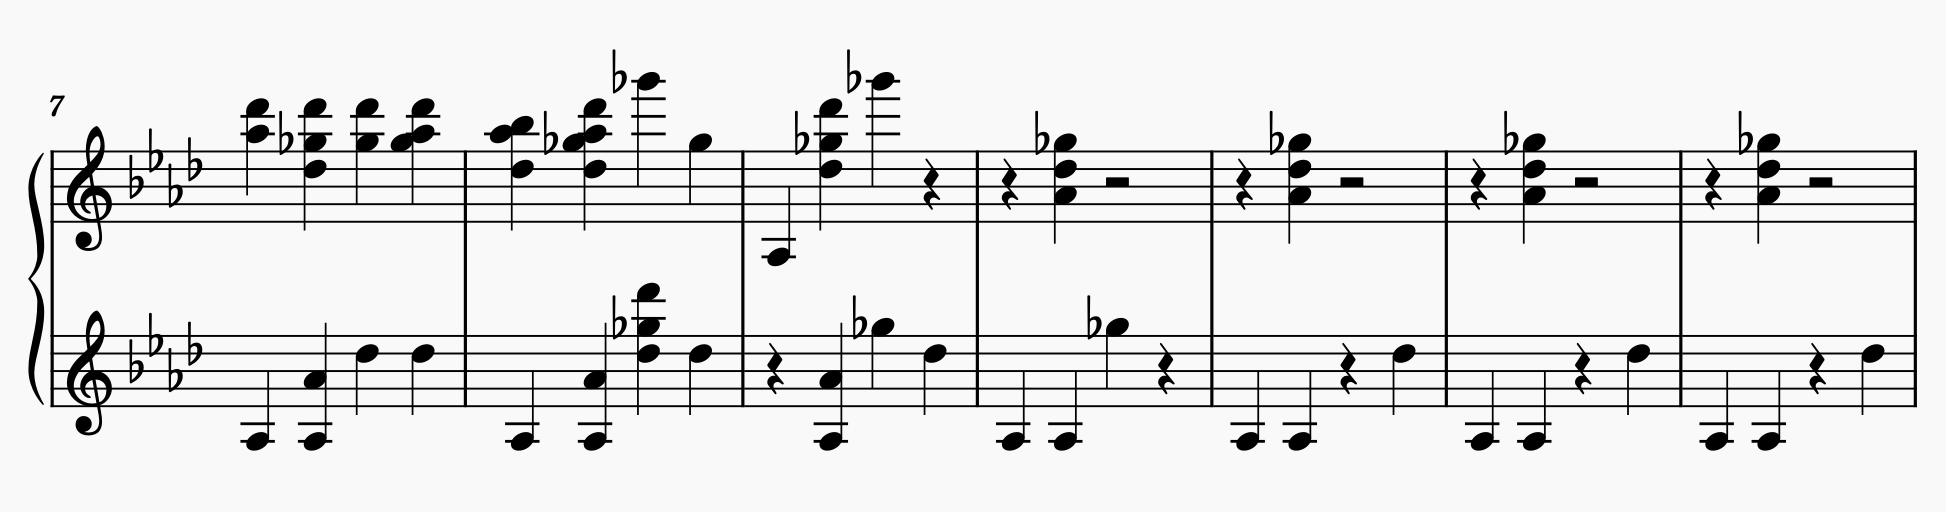
\includegraphics[width=0.7\linewidth]{images/repeated-output-notes.png}
    \caption{Self-fed output from the simple CNN after feeding it the first 4 notes of the Wind Waker title theme (also found on \href{https://www.ninsheetmusic.org/browse/series/TheLegendofZelda}{NinSheetMusic}). We can see after the first 3 measures, the notes begin repeating.}
    \label{fig:simplecnn-repeat}
\end{figure*}

\subsubsection{U-Net results}

At first glance, we can see vastly improved performance when reconstructing chords individually from given input (\autoref{tab:cnn-metrics}). It has greatly reduced loss and improved F2 score, but funnily enough, the repeated generation of chords has nearly the same performance as the simple CNN. A possible explanation of this is that despite how sophisticated a network is, if only given four previous chords, there's only so much the network can do to reconstruct a whole song. We see that even U-Net has long term worse performance in this repeated chord generation than the simple CNN (\autoref{fig:cnn-comp}), even though it has better initial performance.

However, like last time, the metrics don't tell the whole story. The inclusion of skip connections and max pooling allows the network to make inferences about the next chord even if the previous chords are sparse and only contain a few notes. In addition, even small changes in the chords can produce vastly different results, since U-Net can capture how subtle differences in the original score evolve the music differently. We can see this effect immediately in \autoref{fig:unet-norepeat}, where even by the end of our generation, there is no obvious repeating behavior compared to how the simple CNN performed on the same song. At most, there are motifs that are repeated, but it is an improvement over a repeated single note or measure.

\begin{figure}
    \centering
    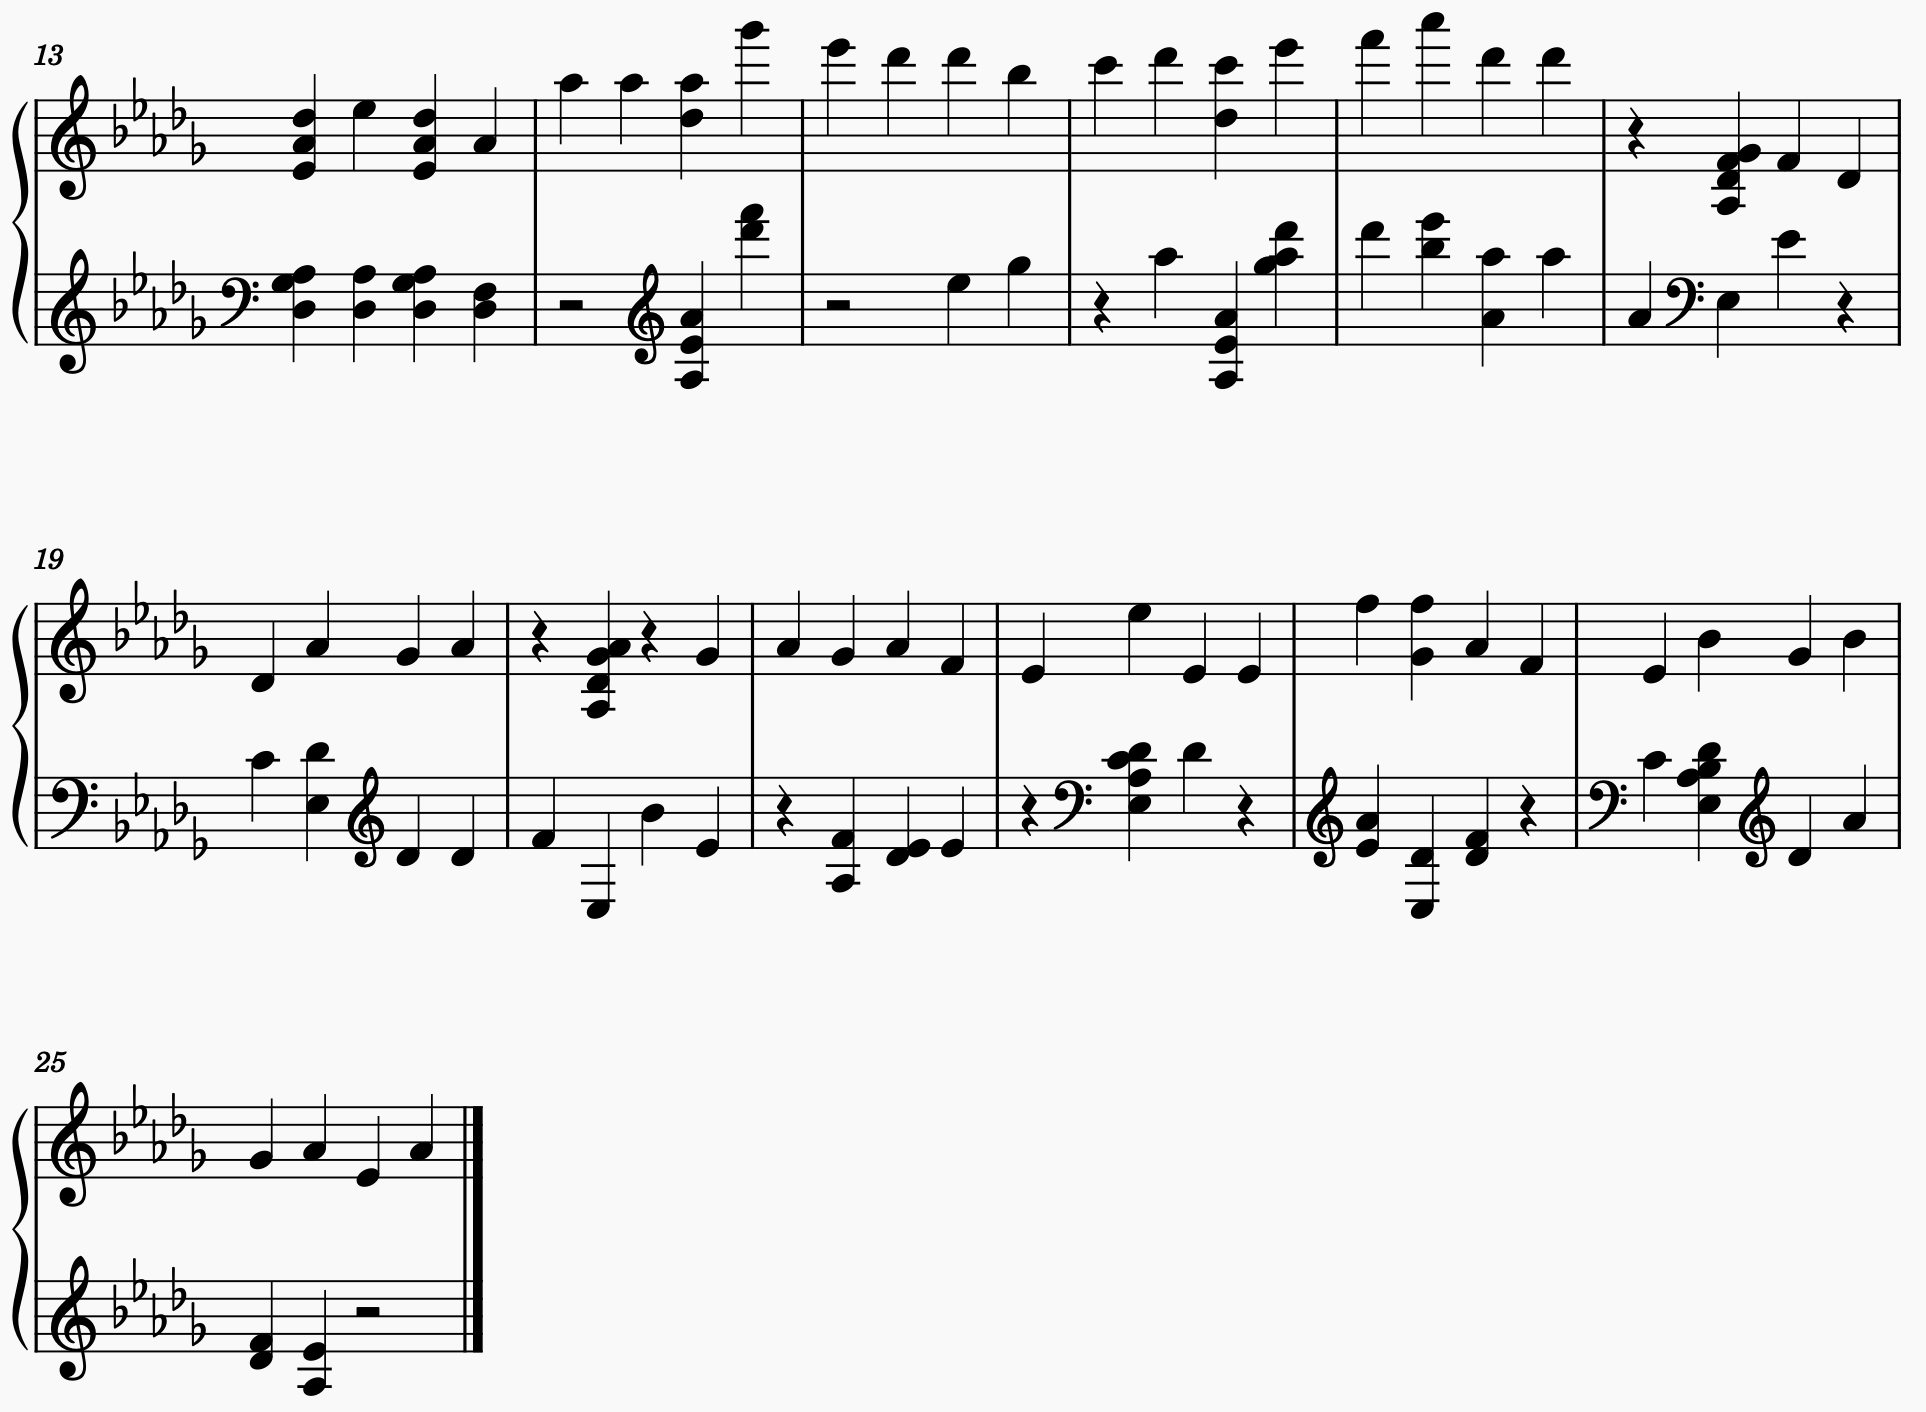
\includegraphics[width=\linewidth]{images/windwaker-unet.png}
    \caption{Self-fed output from U-Net after feeding it the first 4 notes of the same Wind Waker title theme. We can see that even by the end of the song, there are no obvious repeating chords, and the overall chord progression matches somewhat with the original song.}
    \label{fig:unet-norepeat}
\end{figure}

\subsubsection{Miscellaneous tests: key changes and song extensions}

These other tests are slightly outside the scope of the prediction tasks of the models, but intuitively, should produce feasible results. In particular, there are no ways to evaluate the quality of extensions to the end of songs because there is no truth, so instead for these experiments, we will evaluate them qualitatively on a particular song.

We first look at how the networks perform when there is a key change in the input songs. In other words, every note is shifted a certain number of semitones. In theory, since convolutions only capture local Tonnetz note behavior, the networks should be able to generate further songs in the new key. However, in \autoref{fig:gerudo-keychange}, we can see that U-Net fails to reflect this change in behavior, but the simple CNN does. The original song is written in A-major, and we can see U-Net immediately converges back to that key even though the fed input was shifted down 4 semitones. However, in the simple CNN, it continues to generate music in the key of F-major, which is the correct new key. This is a strong sign of something akin to overfitting happening in U-Net due to the skip connections and downsampling. The max-pooling during encoding reduces the dimension of the Tonnetz graph to the point where any sign of a key change disappears. The skip connections are overfitted to the original music so any sequential predictions converge quickly back to the original key.

Next, we look at the differences in the networks when extending from the end of the song in \autoref{fig:gerudo-extension}. Since there is no quantitative way to measure any metric, this has to be evaluated on an individual basis. Alternatively we can compare the complexity/behavior of the extension to the original song by observing its note distribution, but due to time constraints, we do not have this metric. We can see both networks start off similarly but diverge slightly to different parts of the original song in previous measures. This is expected since we don't have any randomness to create novel chords, so it is based purely off what the network was trained off of. Listening to the music manually, the new chords are certainly accurate to the chord progression and motifs of the original song, but are ultimately not novel chords.

\begin{figure}
    \centering
    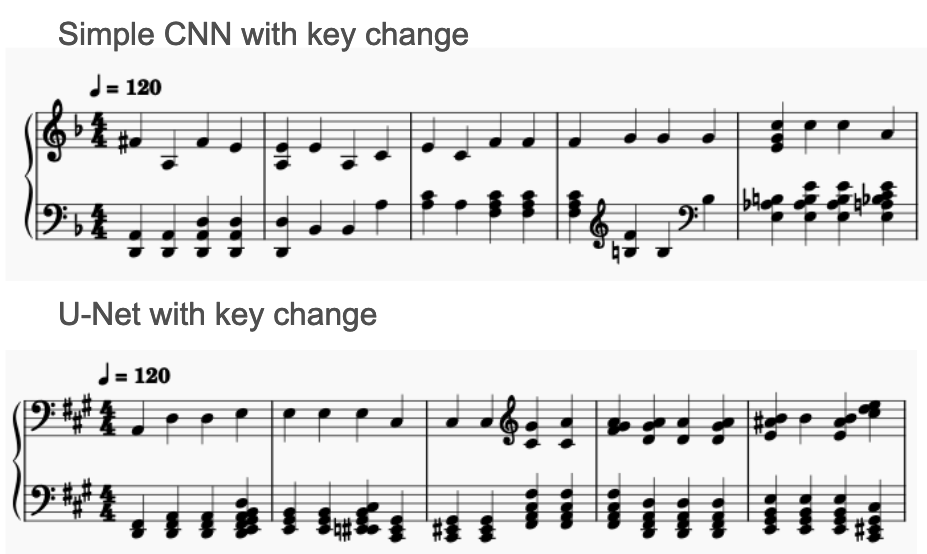
\includegraphics[width=\linewidth]{images/gerudo-keychange.png}
    \caption{Comparison of the first 5 measures between the simple CNN and U-Net when generating from the first 4 chords of the Gerudo Valley theme, shifted down by 4 half-steps.}
    \label{fig:gerudo-keychange}
\end{figure}

\begin{figure}
    \centering
    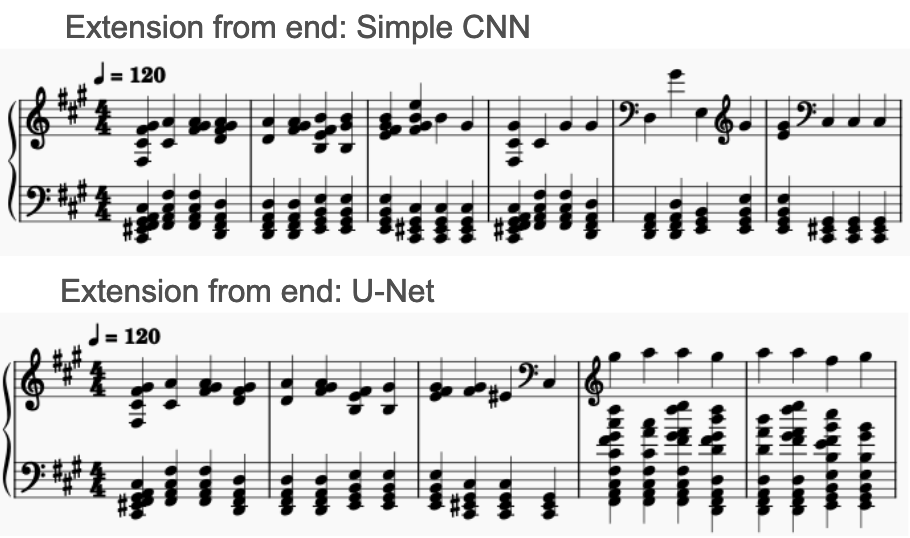
\includegraphics[width=\linewidth]{images/gerudo-extension.png}
    \caption{Comparison of the first 5 measures between the simple CNN and U-Net when generating from the last 4 chords of the Gerudo Valley theme.}
    \label{fig:gerudo-extension}
\end{figure}

\section{Conclusion and potential future paths}

As a result of our experiments, we can see that the task of predicting new chords can be done using Tonnetz graph representations. First with completely synthetic music in the form of cellular automaton, which is highly unstable in its creation of new musical chords, yet can still create some measures of music that make sense tonally. In terms of convolving the Tonnetz data, we find that with simply structured convolutional networks, it can create valid tonal chords common in many musical scores, while the network itself has no direct knowledge of tonal relations between the notes. All of that information is provided inherently by the format of our data in the form of a Tonnetz grid, allowing us to simplify models. We also test with a more complex model like U-Net, which yielded robust results that tend towards the original song regardless of input.

Further potential work in the generation of novel chords can probably be done similarly to how diffusion models create images, in the way that we add noise to the Tonnetz graph in steps and denoise it to create new chords according to a training set. This method could prove effective in not only predicting notes in the songs, but also repairing missing measures of music or creating something completely novel due to the inherent noise in the methods.

\section{Software availability}

All the code used can be found at this GitHub link: \url{https://github.com/jerukan/tonnetz-ece227-final}.

\section{Effort contribution}

This project was done solo, by me.

%----------------------------------------------------------------------------------------
%	 REFERENCES
%----------------------------------------------------------------------------------------

\printbibliography % Output the bibliography

%----------------------------------------------------------------------------------------

\end{document}
